% Template for Carleton problem sets
% Author: Andrew Gainer-Dewar, 20131
\documentclass[twoside]{article}
\usepackage{ccpset}
\usepackage{graphicx, pdfpages}
\usepackage{fixltx2e}

% The Latin Modern font is a modernized replacement for the classic
% Computer Modern. Feel free to replace this with a different font package.
\usepackage{lmodern}

%\titleformat{\subsection}[runin]{}{}{}{}[]

\title{EE445L - Lab 07 Report}
\author{Kevin Gilbert\\ Gilberto Rodriguez}
\date{March 28 2014}
\prof{Professor Bard}
\course{Lab: Monday/Wednesday 5-6:15}

\begin{document}
\raggedbottom
\maketitle{}

\section{Requirements Document}
\subsection{Overview}
\subsubsection{Objectives}
Our project will be centered around developing a board to form the basis of a teleoperated car. The primary goal is to develop an RC car that will communicate wirelessly with a ZigBee and use onboard sensors to allow a level of self-control.
\subsubsection{Roles and Responsibilities}
This device is aimed towards DIY and hobbyist groups, as well as high school and college level robotics teams. Gilbert and I will design the circuit schematic and software design layout as a group. PCB routing will be handled primarily by a single person, as it is difficult to share work during this process. The software realization will be written by both of us as well.
\subsubsection{Interactions with Existing Systems}
We will be using the LM3S1968 board as a controller for our device, using a ZigBee.
\subsection{Function Description}
\subsubsection{Functionality}
The system will have an on-board LM3S811 chip to collect data from the ZigBee and interface with the motors. The embedded device will also include motor controllers for actuation, and onboard sensors to allow a degree of autonomity. A power regulator will allow for battery operation.
\subsubsection{Performance}
ISR lengths through debugging instruments. Current needed to power board with and without motors running.
\subsubsection{Usability}
The LM3S1968 will be used to broadcast the wireless signal to the car. User input will be captured using button inputs, and the car's speed will displayed through either a set of 7-segment displays or the onboard OLED.
\subsection{Deliverables}
\subsubsection{Reports}
We will write a report for Labs 7 and 11.
\subsubsection{Outcomes}
\bf{Lab07:}
\begin{enumerate}
\item 1-page requirements document
\item Hardware Design: Regular circuit diagram (SCH file) PCB layout and three printouts (top, bottom and combined)
\item Software Design: Include the requirements document (Preparation a)
\item Measurement Data: Give the estimated current (Procedure d). Give the estimated cost (Procedure e)
\item Analysis and Discussion (none)
\end{enumerate}

\noindent \bf{Lab11:}
\begin{enumerate}
\item Objectives: 2-page requirements document
\item Hardware Design :Detailed circuit diagram of the system (from Lab 7)
\item Software Design (no software printout in the report): Briefly explain how your software works (1/2 page maximum)
\item Measurement Data: As appropriate for your system. Explain how the data was collected.
\item Analysis and Discussion (1 page maximum) 
\end{enumerate}

\section{Hardware Design}
	\subsection{Circuit Schematics}
		\subsubsection{Control Circuit}
			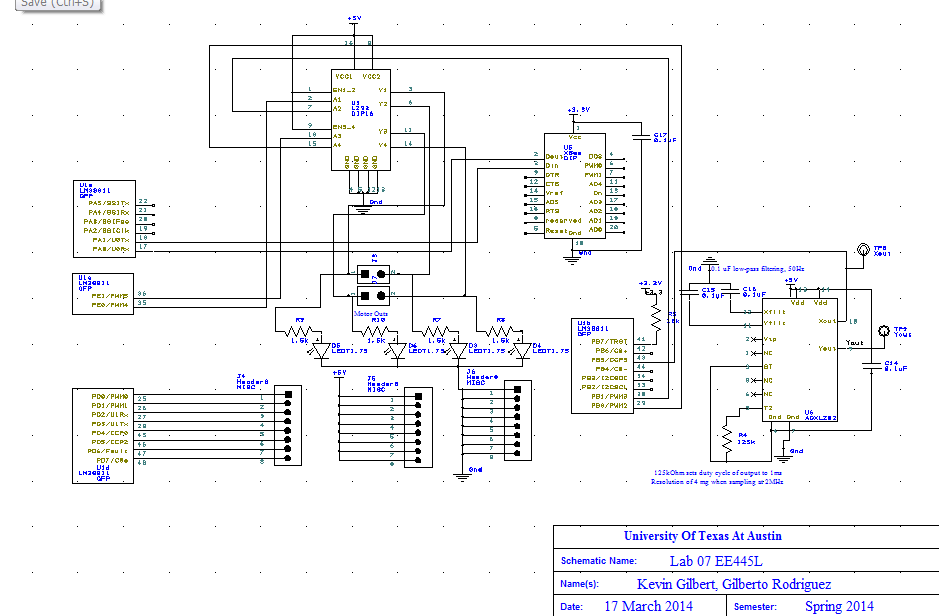
\includegraphics[width=\textwidth]{circuitDiagram}
		\subsubsection{Power Circuit}
			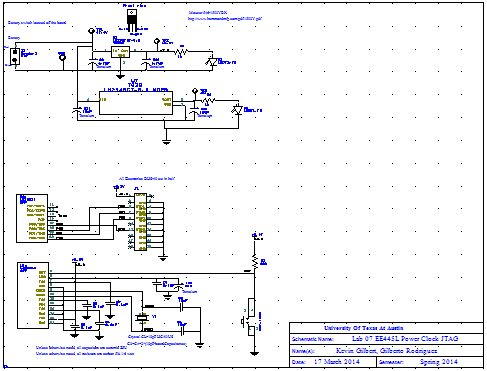
\includegraphics[width=\textwidth]{powerCircuit}
            
    \subsection{PCB Design}
    	\subsubsection{PCB Top Copper}
        	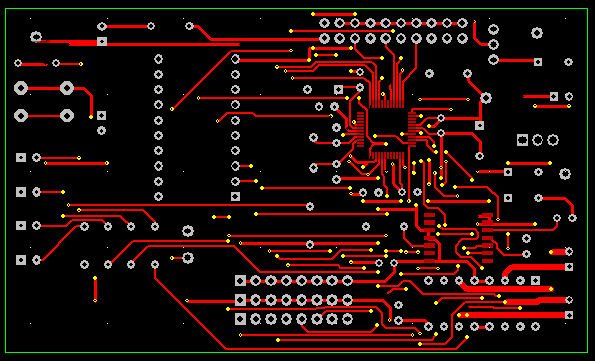
\includegraphics[width=\textwidth]{topCopper}		
		\subsubsection{PCB Bottom Copper}
       	    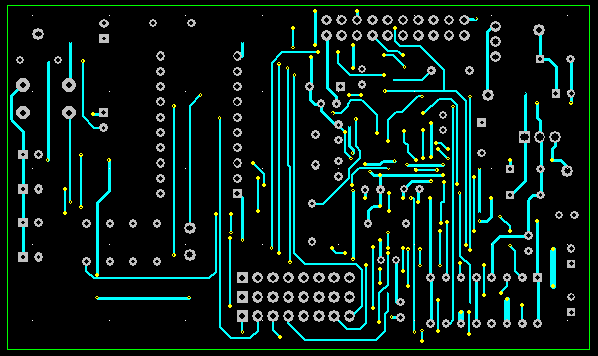
\includegraphics[width=\textwidth]{bottomCopper}  
    	\subsubsection{Total PCB}
        	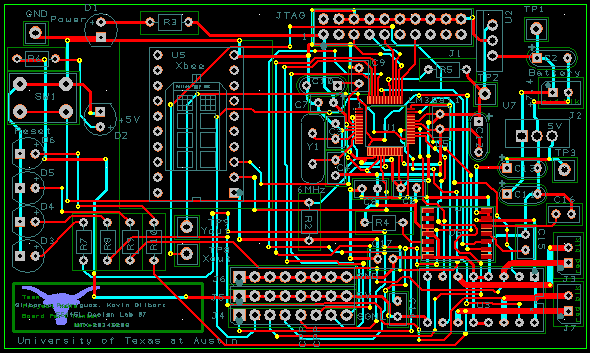
\includegraphics[width=\textwidth]{pcb}
            
\section{Software Design}
Through testing, we discovered no major flaws in the design.

\section{Measurement Data}
Estimated Current: 600 mA \\
Estimated Cost: \$34.70 for parts + \$53.00 for board (including shipping) = \$87.70 \\
\$20.00 overall (with free samples)
 
\end{document}